
\textbf{ŞABLONU KULLANMAK İÇİN ÖNCE PROJE TÜRÜ SEÇMELİSİNİZ}

Main.tex dosyasını açınız, 38. satırdaki değeri aşağıdaki kurallara göre değiştiriniz\\
Bu dosyada aşağıdaki kısımdaki {} değeri değiştirmeniz yeterlidir\\
\\
 Halihazırda \textbf{"projecttype değişkenindeki 0"} olan ilgili değeri;  \\
 AR-GE PROJELERİ için 1,\\
 YAZILIM PROJELERİ için 2 \\
 LATEX TUTORIAL için 3 olarak değiştiriniz.

\begin{figure}[H]
    \centering
    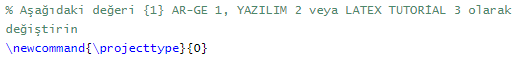
\includegraphics[width=0.8\linewidth]{LatexTutorial/image_2024-09-11_112818430.png}
    \caption{PROJE TÜRÜ SEÇİMİ}
    \label{fig:enter-label}
\end{figure}




\textbf{TO USE THE TEMPLATE, YOU MUST FIRST SELECT THE PROJECT TYPE}

Open the Main.tex file and change the value on line 38 according to the following rules.\\ It is sufficient to change the value in the {} section below.\\

Currently, change the relevant value in \textbf{"the projecttype variable which is 0"} to: \\ 1 for R\&D PROJECTS, \\ 2 for SOFTWARE (SW) PROJECTS, \\ 3 for LATEX TUTORIAL. \begin{figure}[H] \centering 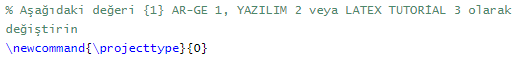
\includegraphics[width=0.8\linewidth]{LatexTutorial/image_2024-09-11_112818430.png} \caption{PROJECT TYPE SELECTION} \label{fig:enter-label} \end{figure} 